\section{Implementation}
Kaptitel beschreibt die implementation

\begin{figure}[H]
  \begin{center}
    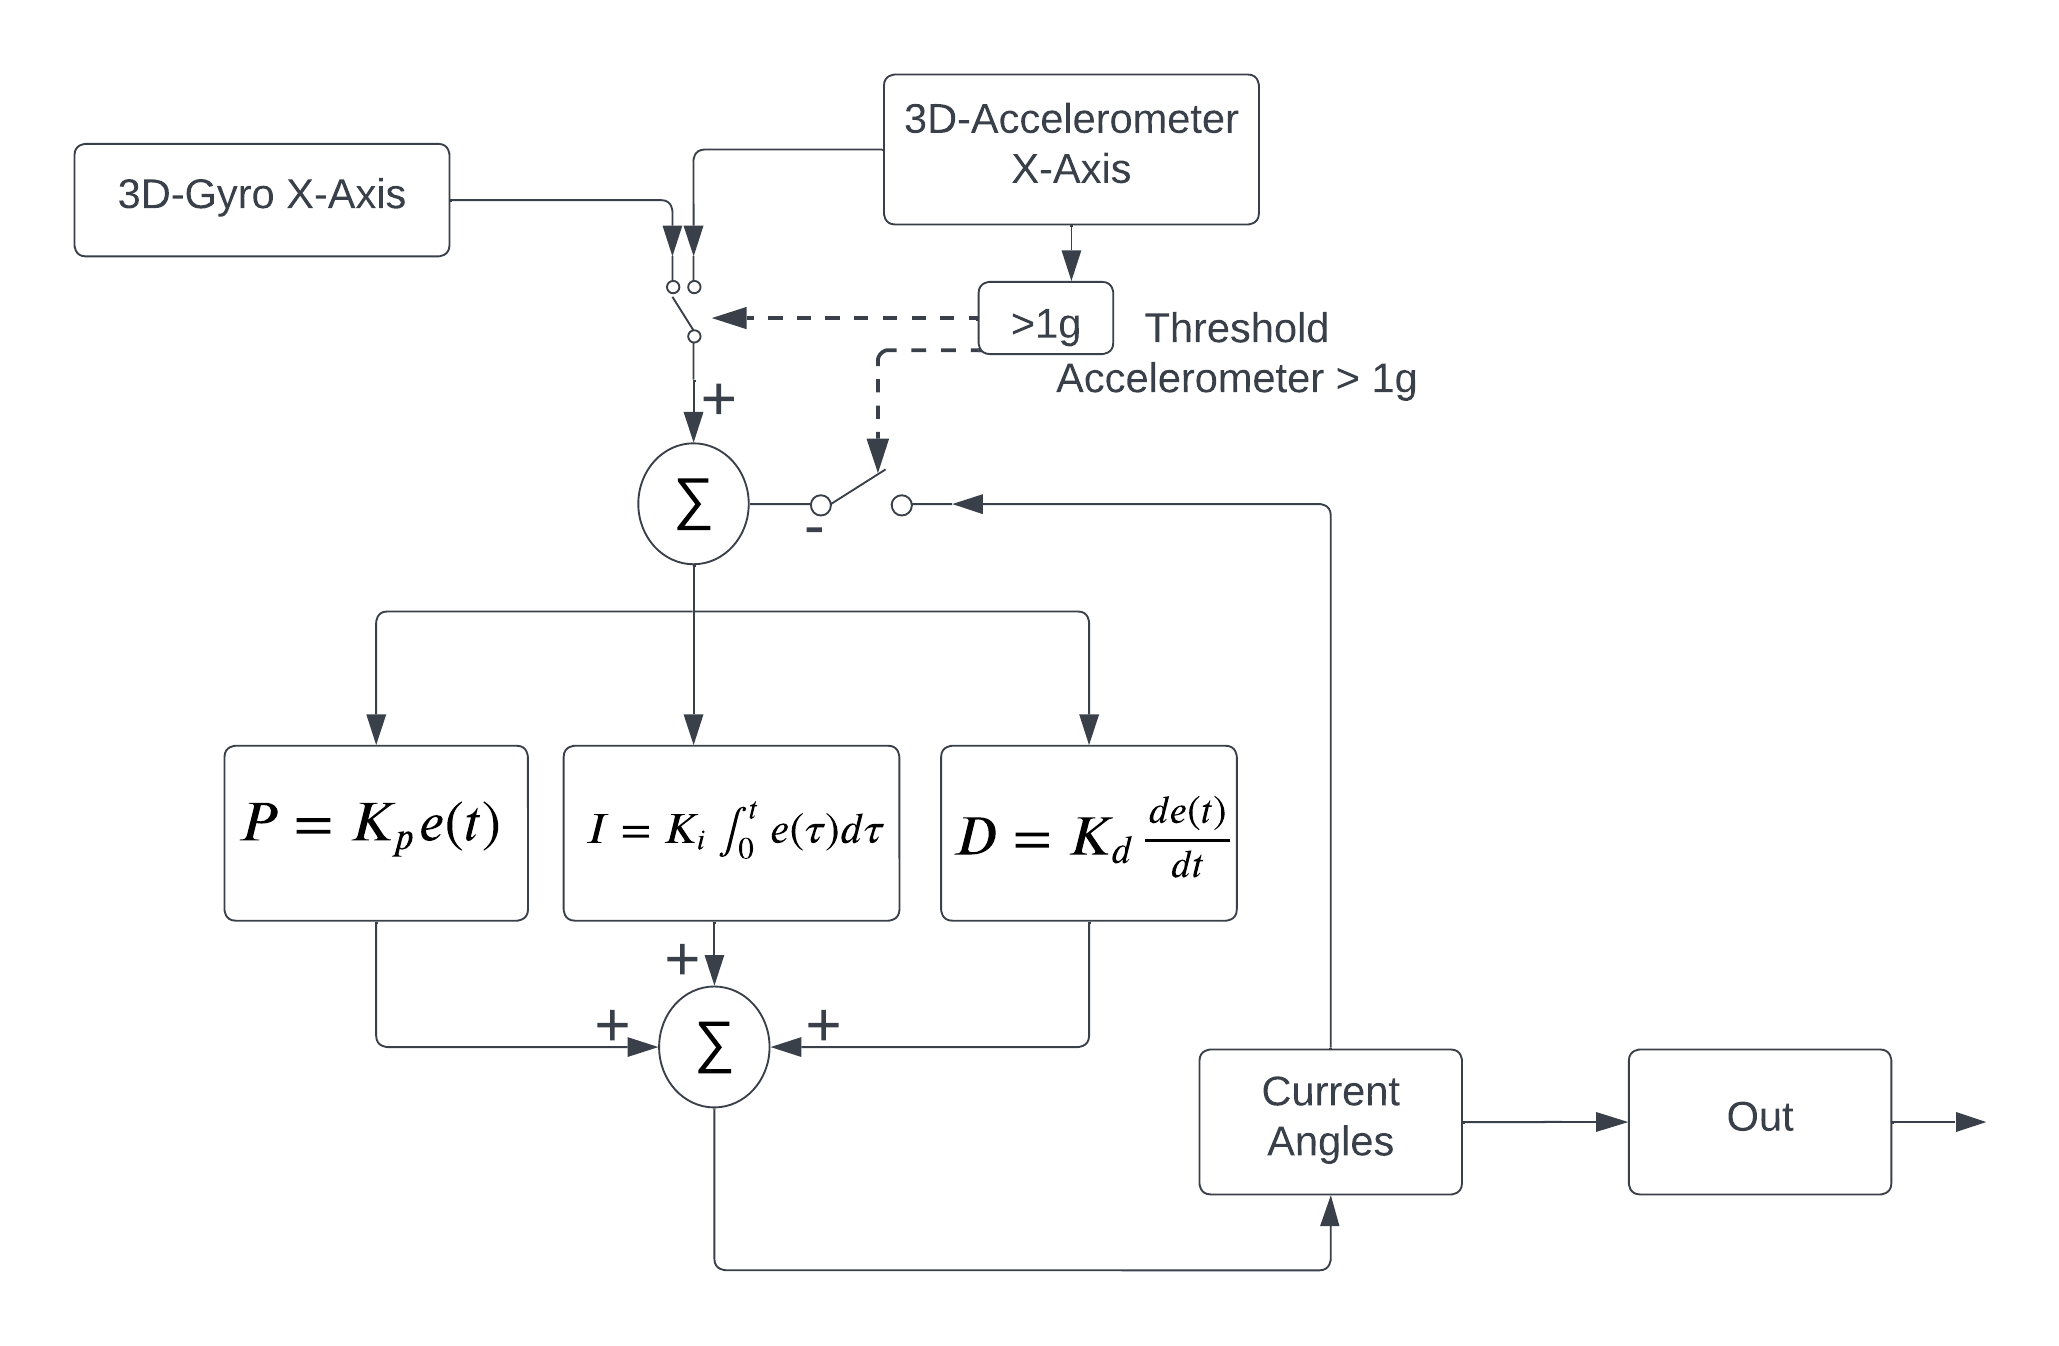
\includegraphics[width=1\linewidth]{content/images/PID_Loop.png}
    \caption{PID Loop}
  \end{center}
\end{figure}

\subsection{UseCase}
\begin{figure}[H]
  \begin{center}
    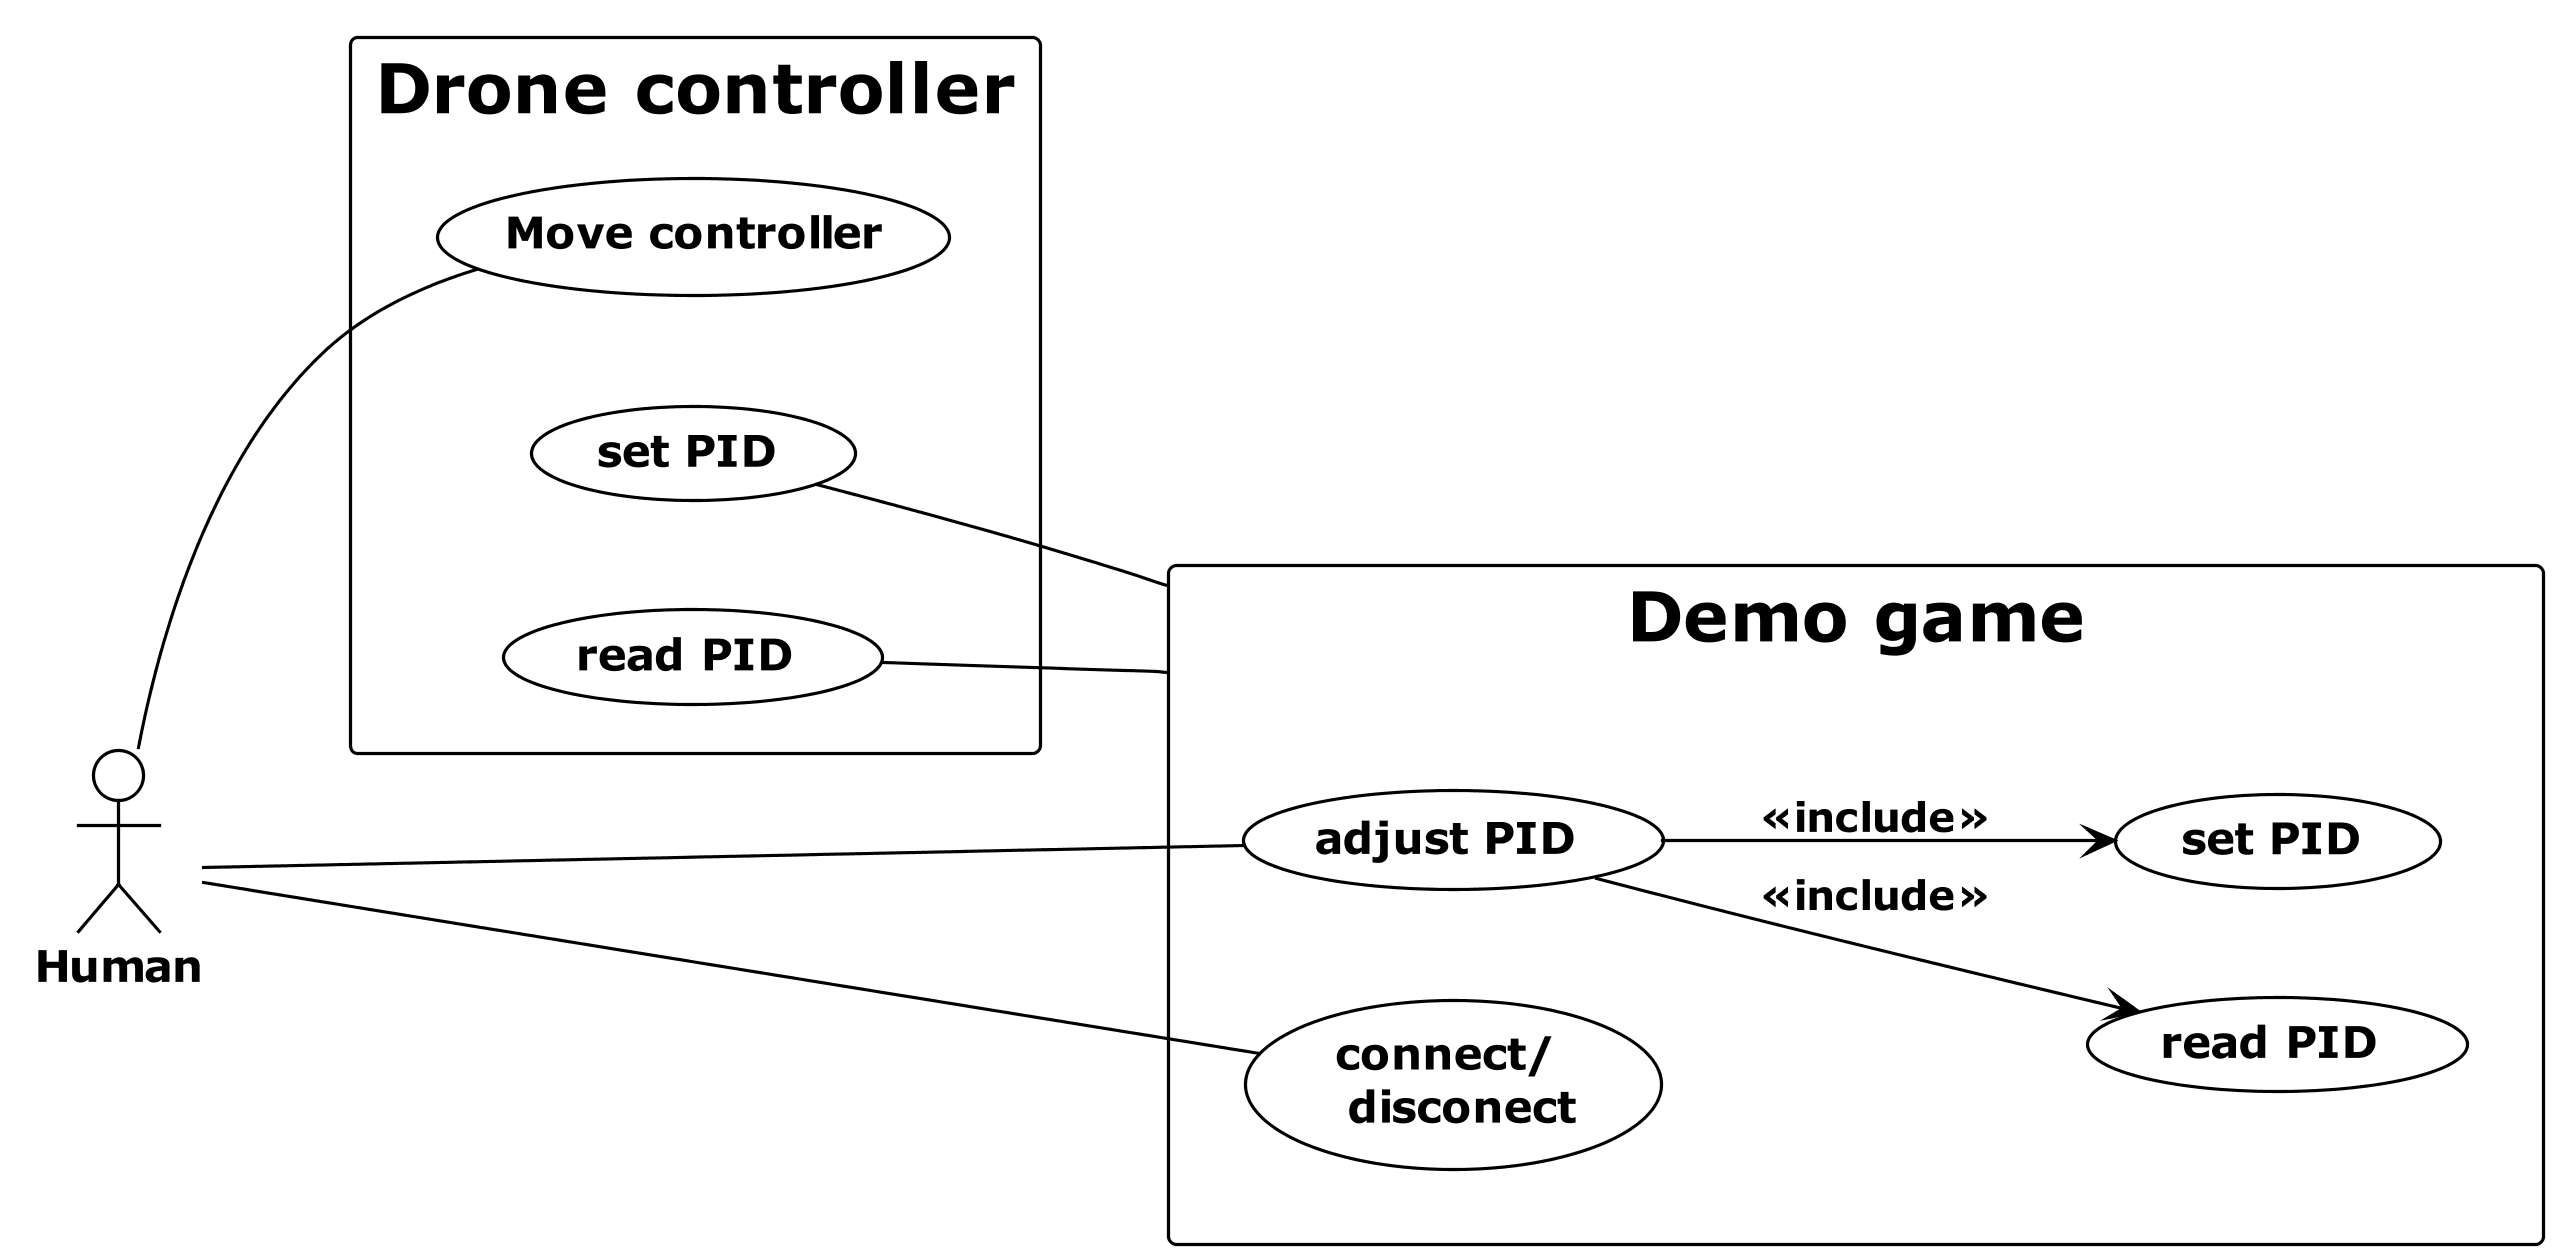
\includegraphics[width=0.8\linewidth]{content/diagrams/out/usecase/sendAngles.png}
    \caption{Send angles}
  \end{center}
\end{figure}

\subsection{Sequenzdiagramme}
\begin{figure}[H]
  \begin{center}
    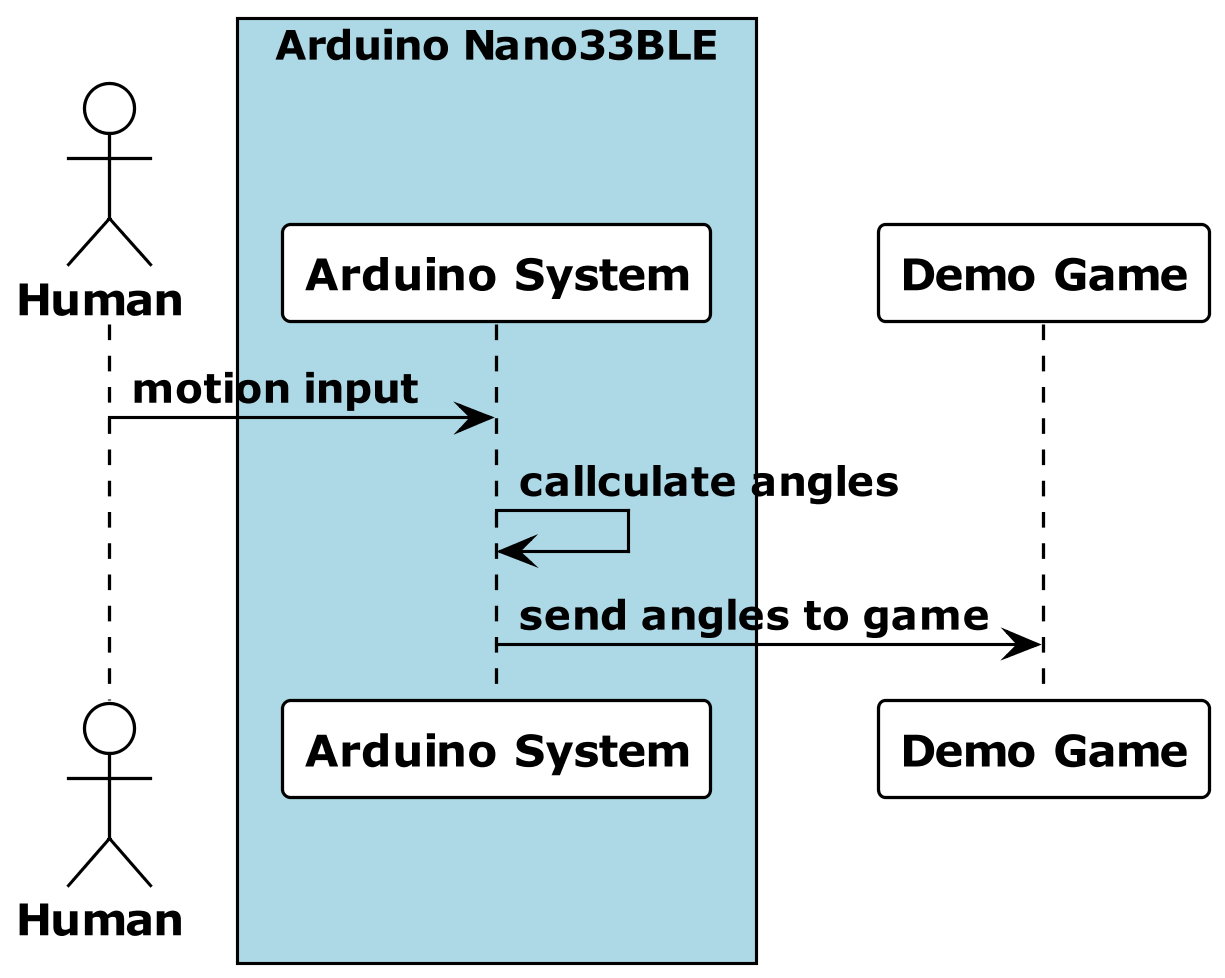
\includegraphics[width=0.7\linewidth]{content/diagrams/out/sequence/system.png}
    \caption{System}
  \end{center}
\end{figure}

\begin{figure}[H]
  \begin{center}
    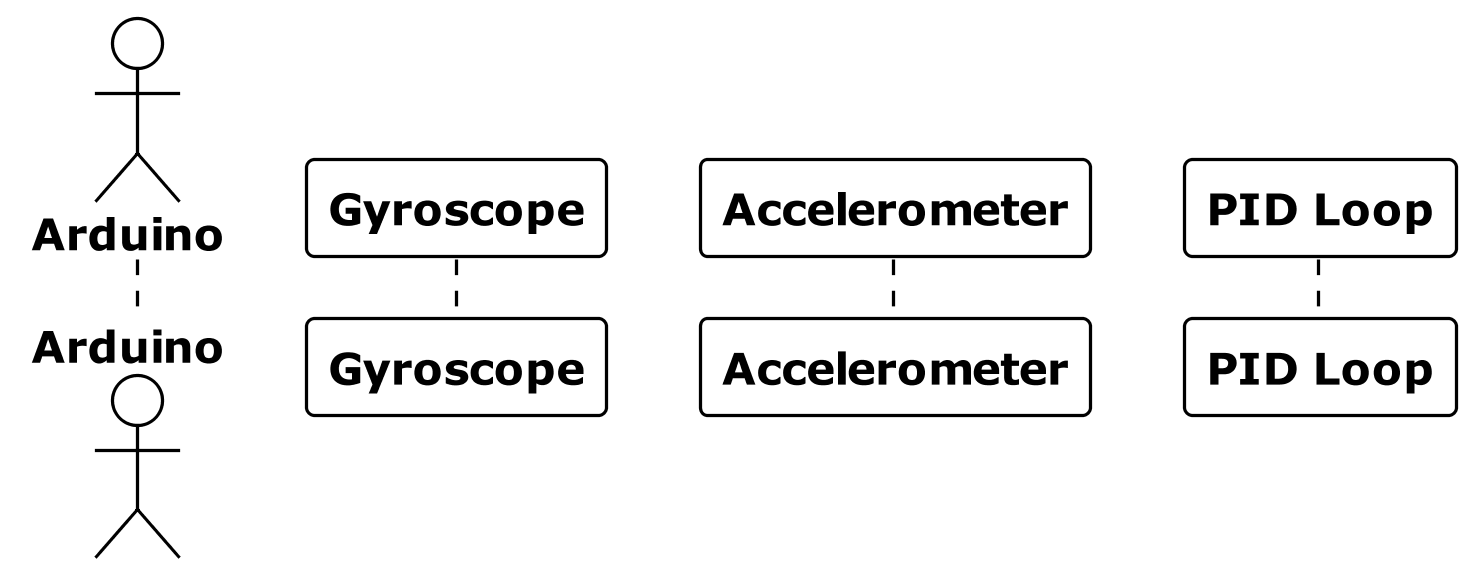
\includegraphics[width=0.8\linewidth]{content/diagrams/out/sequence/arduino.png}
    \caption{Arduino}
  \end{center}
\end{figure}

\begin{figure}[H]
  \begin{center}
    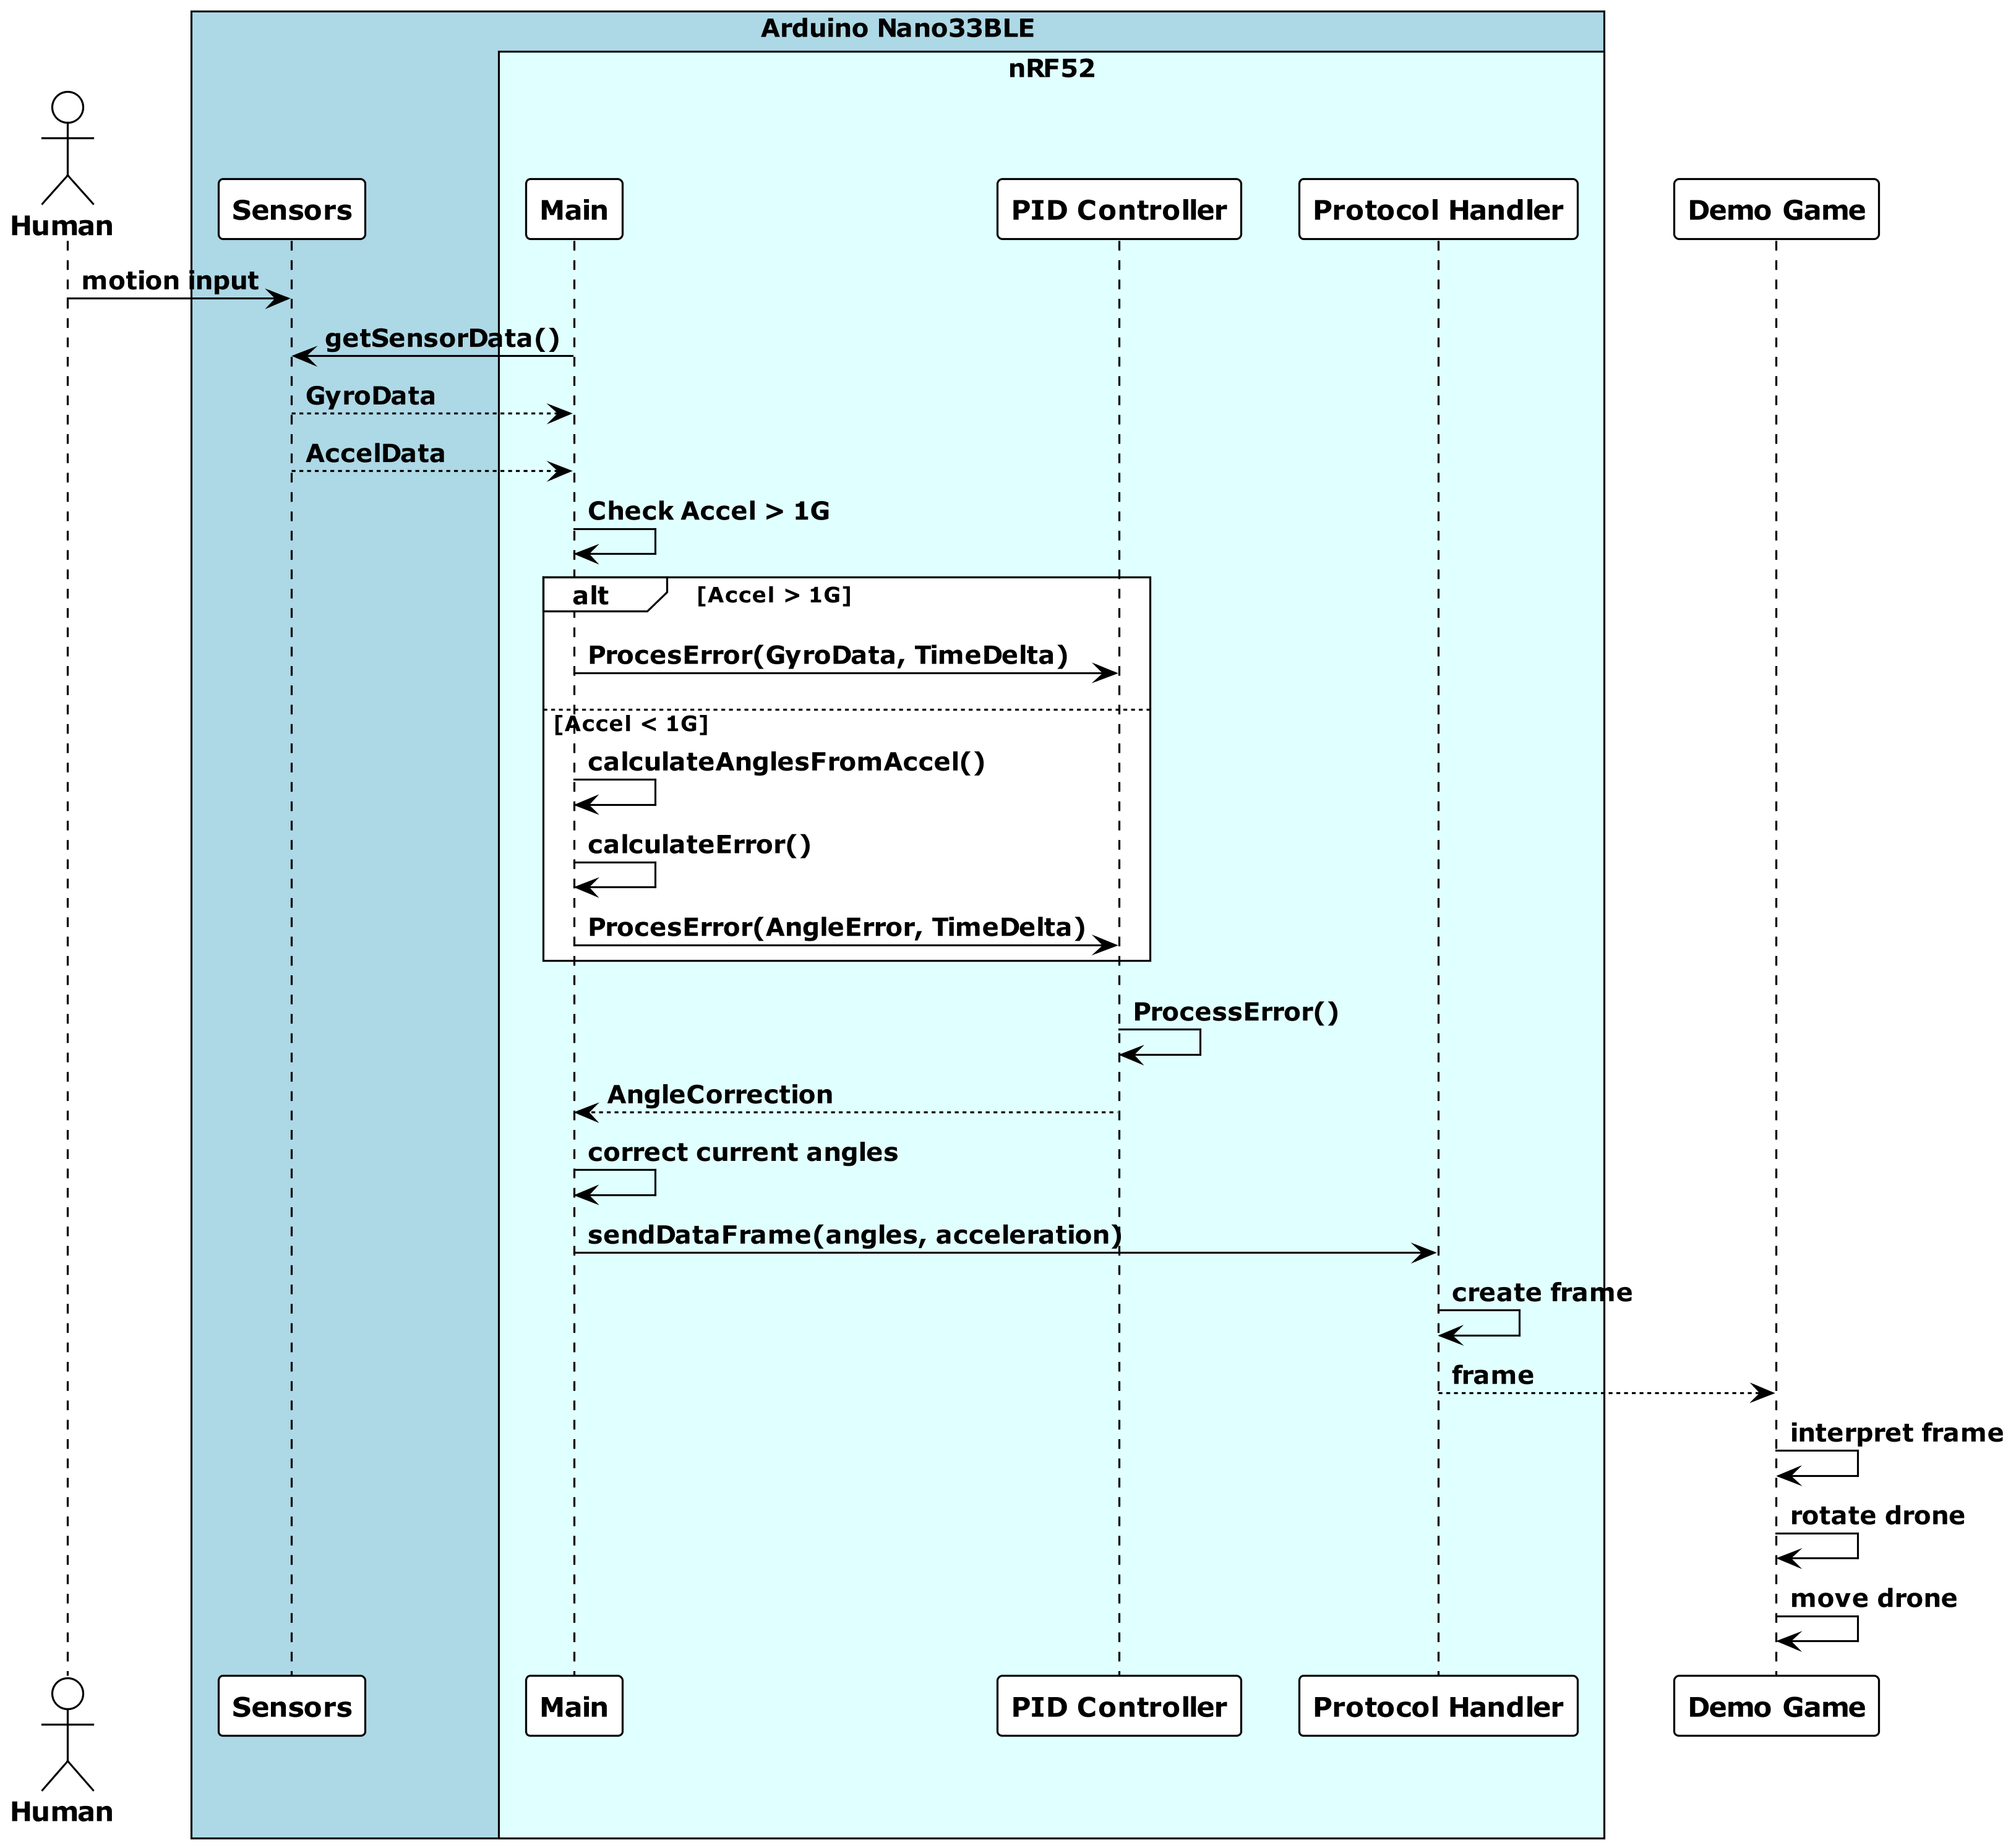
\includegraphics[width=0.8\textheight]{content/diagrams/out/sequence/moveController.png}
    \caption{Move controller}
  \end{center}
\end{figure}

